\documentclass[graphics]{beamer}

\usepackage{graphicx}
\usepackage{verbatim}
\usepackage{wrapfig}
\useoutertheme{shadow}
%\usecolortheme{orchid}
\usecolortheme{seahorse}


% math commands
\newcommand{\be}{\begin{eqnarray}}
\newcommand{\ee}{\end{eqnarray}}
\newcommand{\beq}{\begin{equation}}
\newcommand{\eeq}{\end{equation}}
\def\simless{\mathbin{\lower 3pt\hbox
      {$\rlap{\raise 5pt\hbox{$\char'074$}}\mathchar"7218$}}}
\def\simgreat{\mathbin{\lower 3pt\hbox
      {$\rlap{\raise 5pt\hbox{$\char'076$}}\mathchar"7218$}}} %> or of order

% variables

\def\toonscale{0.45}
\def\mboxy#1{\mbox{\small #1}}


\begin{comment}
\AtBeginSection[]{
  \frame{
    \frametitle{Outline}
    \tableofcontents[currentsection]
  }
}
\end{comment}

\title{Coherent Lensing: FRBs, GWs, path integrals and effervescent images
}
%\subtitle{interim update}
\author[U. Pen]{Ue-Li Pen, Dylan Jow, Job Feldbrugge
}
\date{November 10, 2023}


\begin{document}

%\section*{Introduction}
\section{Lenses}

\begin{comment}
  \subsection{Outline}

  \frame{
    \frametitle{Outline}
    \tableofcontents
  }
\end{comment}

\frame{\maketitle}


  \frame{
    \frametitle{Gravitational Waves, Fast Radio Bursts}
    \begin{itemize}
        \item Coherent, distant source of radiation
        \item Interference effects under multi-path propagation
        \item potential for diffraction limited measurements
        \item Kirchoff-Fresnel path integral
        \item semi-classical concepts: stationary phase, Eikonal limit
        \item Witten 2010: generalized by Picard-Lefschetz theory
        \item Morse index, effervescent/complex images: measure time delays in weak lensing
    \end{itemize}
  }


  \frame{
    \frametitle{Morse Index}
    \begin{itemize}
      \tiny
        \item Schneider, Ehlers, Falco (1992)
        \item Dai+Venumadhav 2017
        \item image parity:
        \item 90$^o$ phase shift
        \item more angles ...
    \end{itemize}
\vspace{-0.85in}\hspace{1.5in}\includegraphics[width=3.1in]{Figures/dai17.jpg}
  }

  \frame{
    \frametitle{FRBs}
    \begin{itemize}
        \item Coherent, distant source of radiation
        \item Scintillate under multi-path propagation          
        \item sensitive to ns time delay propagating for gigaparsecs
        \item corresponds to strain $h \ll 10^{-26}$: far exceeds LIGO
        \item highly elongated antenna pattern: sensitive to
          longitudinal modes          
    \end{itemize}
  }


  \frame{
\vspace{-0.25in}
    \frametitle{FRB110523}
 

%\hspace{2.5in}
\includegraphics[width=2.5in]{Figures/scint110523.png}
\includegraphics[width=1.75in]{Figures/corr110523.png}

Masui++ 2015, Nature, 528, 523
  }

  \frame{
%\vspace{-0.25in}
    \frametitle{Scintillometry VLBI}
\hspace{-0.25in}
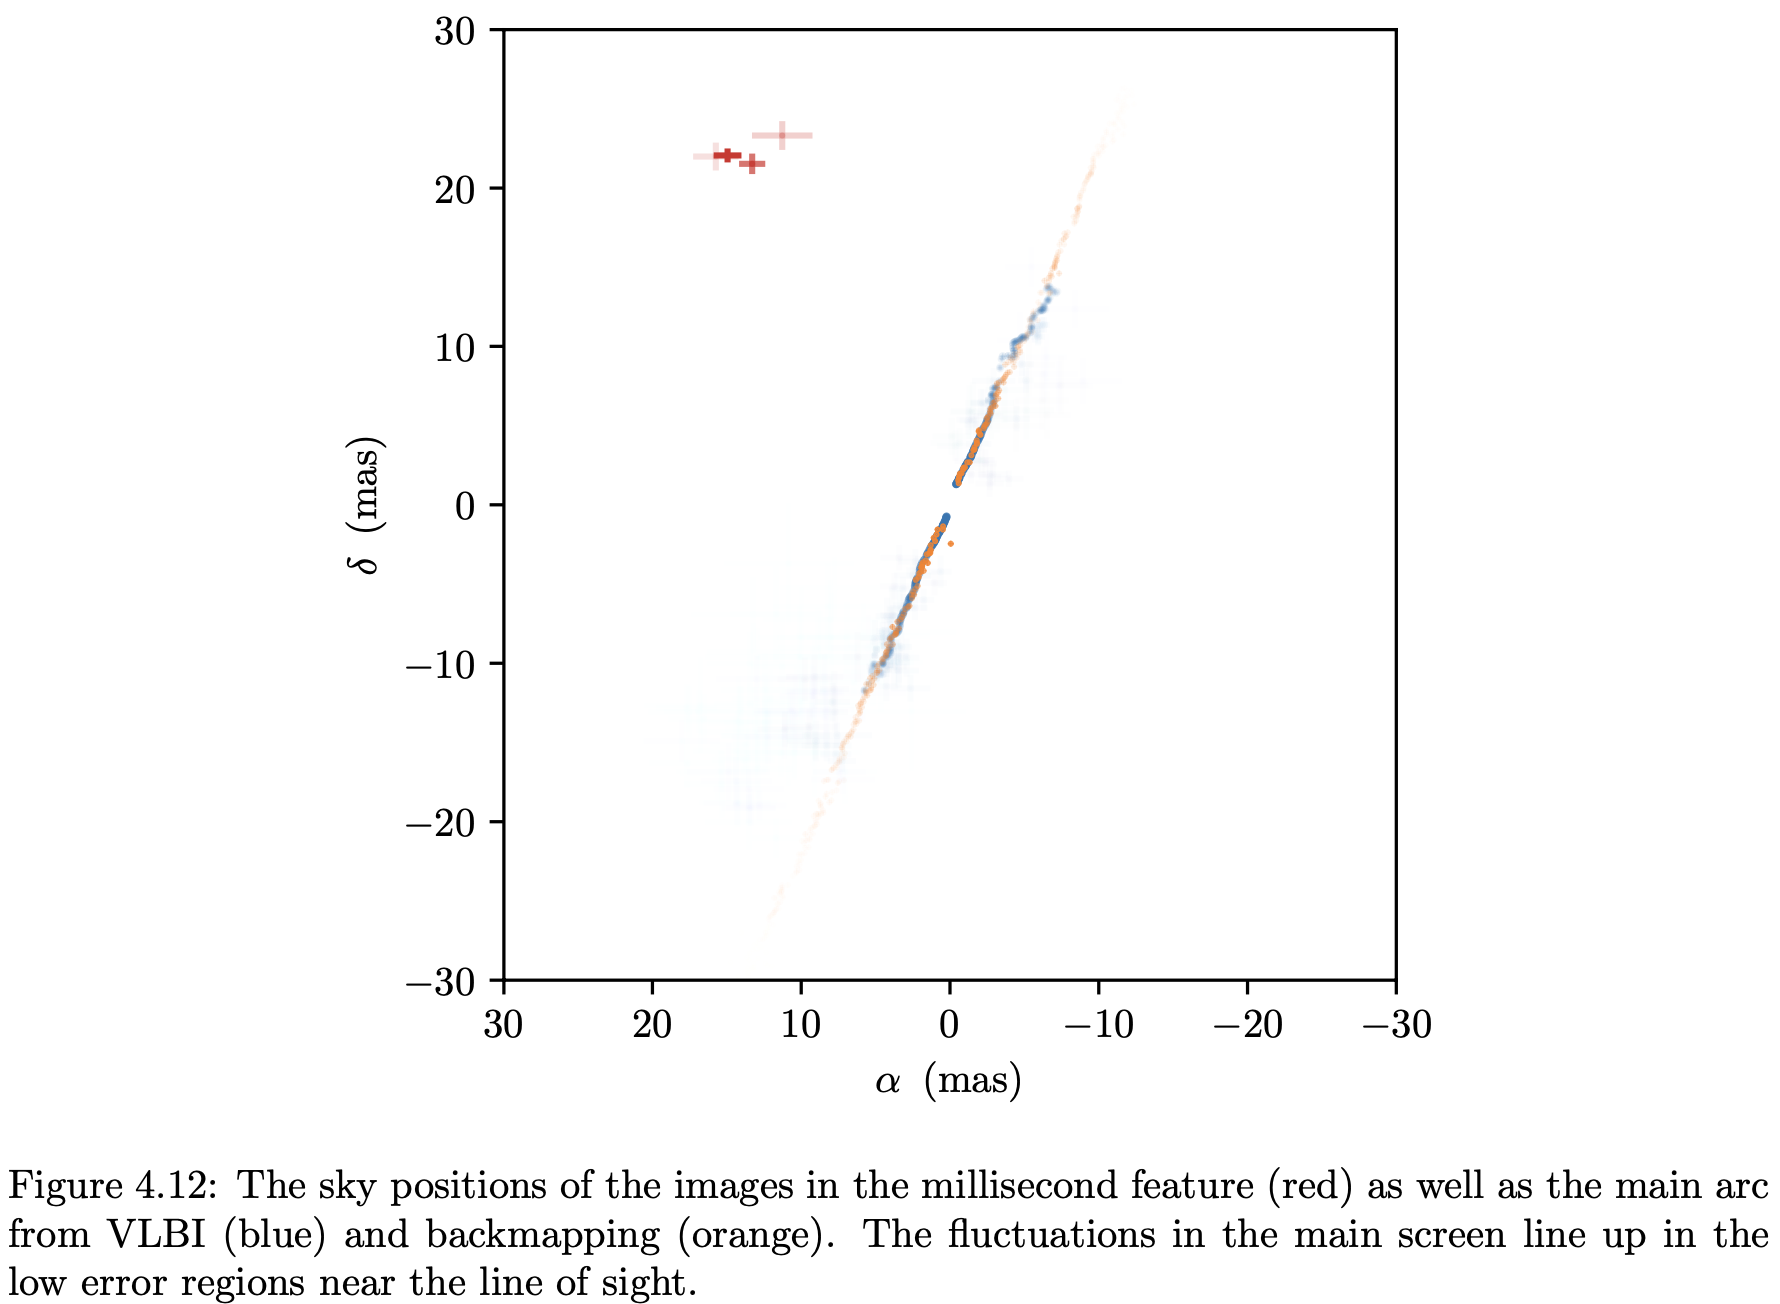
\includegraphics[width=3.5in]{Figures/VLBI0834.png}
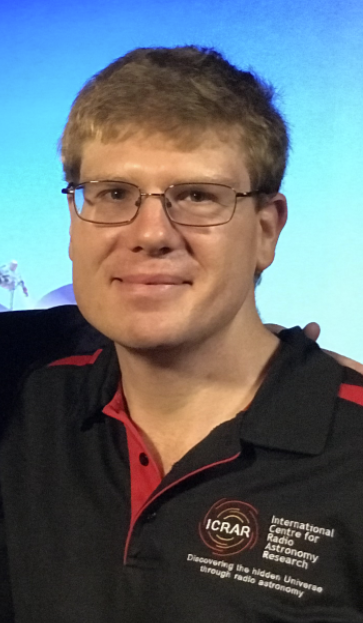
\includegraphics[width=1.05in]{Figures/jpm.png}

Baker++: increase PTA angular resolution to arcminutes.  In memoriam J-P Macquart.
  }



  \frame{

    \frametitle{precision astrometry}
%\vspace{-0.25in}
\begin{center}
%\hspace{-0.5in}
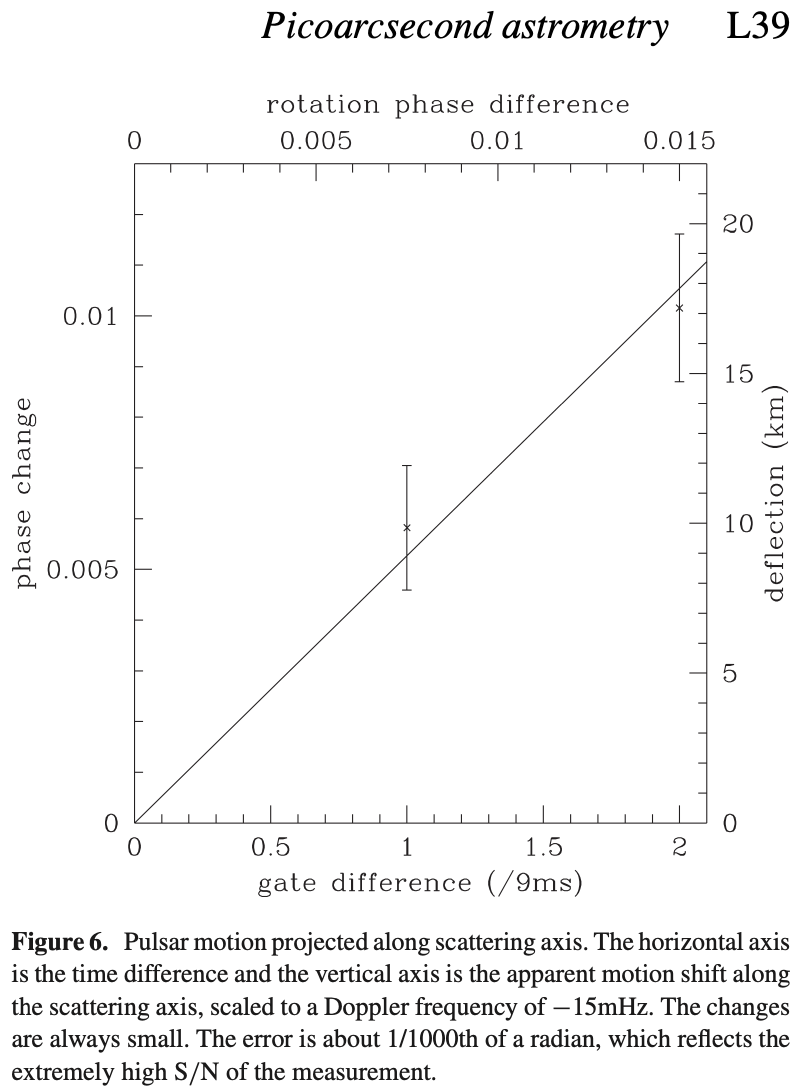
\includegraphics[width=2.05in]{Figures/pico.png}
UP+14
\end{center}
  }


  \frame{
    \frametitle{Waves, Particles, Geodesics}
    \begin{itemize}
        \item Everything is a wave
        \item Short wavelength limit has classical particle
          interpretation: Eikonal
        \item Picard-Lefschetz: no waves, everything is a particle!
        \item effervescent lensing: complex eikonal lensing
        \item New tool for QM Cosmology, FRBs, pulsars
        \item alternative picture for quantization: quantum gravity?
    \end{itemize}
  }


  \frame{
\vspace{-0.25in}
    \frametitle{Fermat's Principle}
    \begin{itemize}
        \item light takes shortest path. Why?
        \item Huygen's principle: light takes all paths
        \item Kirchoff/Feynmann path integral
        \item stationary phase dominates
        \item classical equation of motion: extremal paths, independent of wavelength
\vspace{-0.85in}\hspace{2.5in}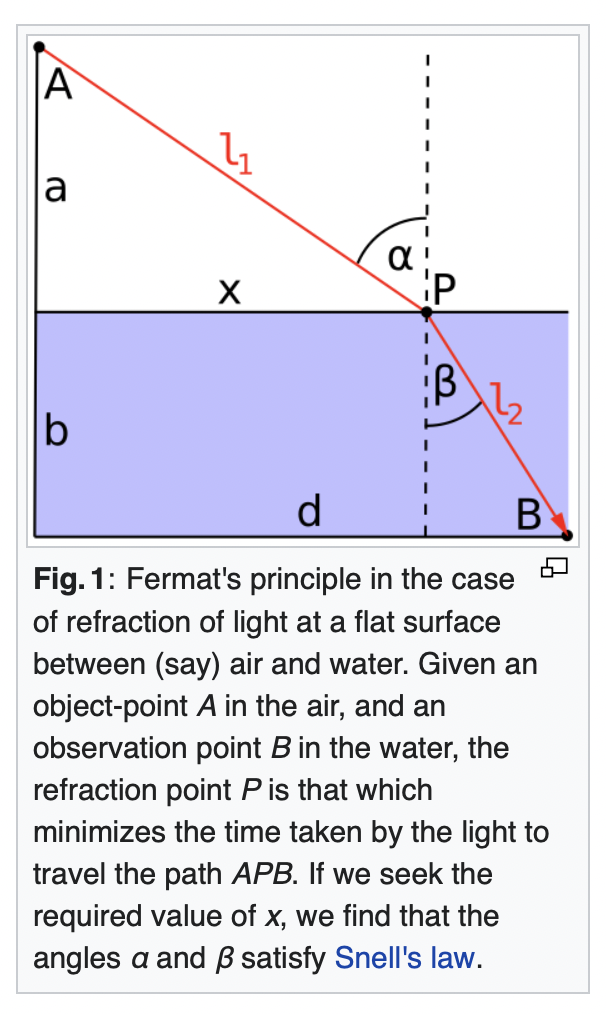
\includegraphics[width=1.3in]{Figures/fermat.png}
    \end{itemize}
  }


  \frame{
\vspace{-0.25in}
    \frametitle{Optics: Geometric, Eikonal, Wave, P-L}
    \begin{itemize}
        \item Consider 1-D lens
        \item lensing potential $\Psi(\theta)$
        \item deflection $\Psi'$
        \item simplify for $D_{\rm ds}=\infty$
    \end{itemize}
\vspace{-0.5in}\hspace{2.5in}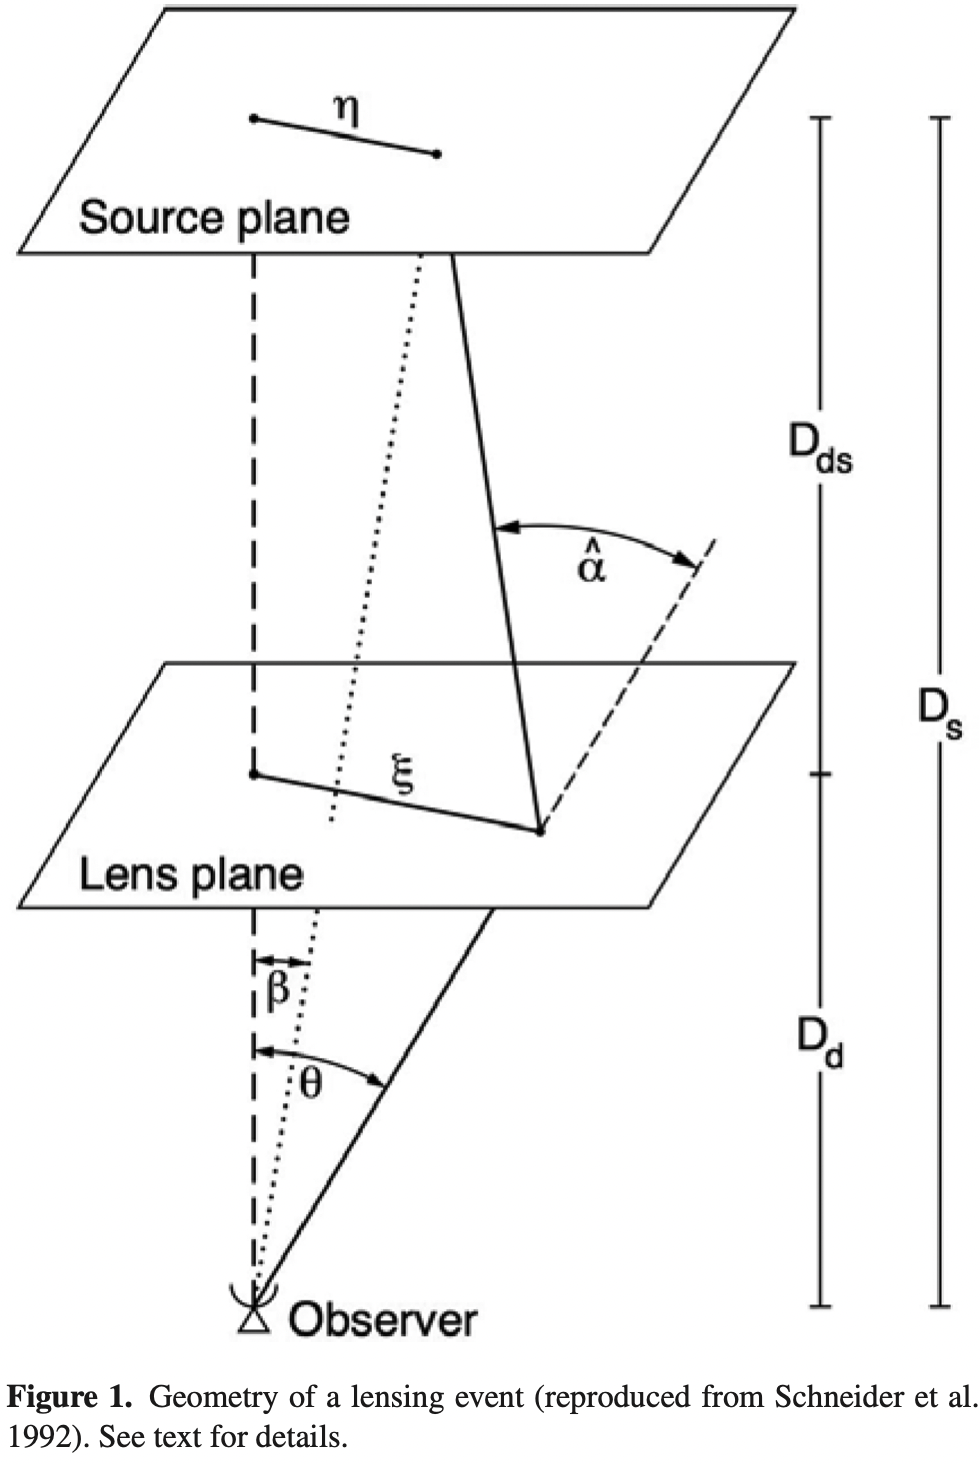
\includegraphics[width=1.5in]{Figures/lens.png}

  }


  \frame{
\vspace{-0.25in}
    \frametitle{Huygen's Principle: Path Integral}
    \begin{itemize}
        \item $A(\mu)=\int e^{i S(\theta,\mu)} d\theta$ 
        \item $S=\nu [(\theta-\mu)^2+\Psi(\theta)]$
        \item Highly oscillatory integral, even for $\Psi=0$
        \item Stationary phase points: $\partial_\theta S=0$ leads to (complex)
          Eikonal images $\theta_i$.
        \item flux/phase through curvature expansion (known as {\it
            steepest descent}): exact as $\nu \rightarrow \infty$
        \item Geometric limit considers only {\it Real} solutions $\theta_i$ and
      gives up phase
          information (length of trajectory)
        \item Geometric optics applicable at short wavelengths for
          extended sources
          (e.g. optical gravitational lensing of finite size sources,
          stars)     
          \item roughly 1/4 of the degrees of freedom of Eikonal 
    \end{itemize}
  }




  \frame{
\vspace{-0.5in}
    \frametitle{Effervescent Images}
    \begin{itemize}
    \item consider ``rational lens'' potential $\psi(\theta)=\alpha/(1+\theta^2)$
    \item Geometric/eikonal images at $\psi'=\theta$
    \item 5 roots.  1 or 3 real roots, rest imaginary
    \item P-L: at most one imaginary image contributes!
    \item Effervescent (imaginary) image can be brighter than unlensed real image
    \end{itemize}
  }


  \frame{
%\vspace{-0.5in}
    \frametitle{Rational 1-D lens}
\begin{center}
\includegraphics[width=3.1in]{Figures/theta-beta.eps}
\end{center}
  }

  
  \frame{
\vspace{-0.5in}
    \frametitle{Picard-Lefschetz Theory}
    \begin{itemize}
    \item descend integral along real line along Morse function Im(S)
    \item contour deforms into finite number of Thimbles of constant
      phase with maximum at saddle point (extrema $dS=0$)
    \item correctly identifies relevant saddle points
    \item resolves numerical challenges of oscillatory integral
    \item complex analysis works in multiple variables
    \item elevates concept of ``image'' deep into wave optics
    \item multiple public implementations (Feldbrugge+, Jow+)
    \end{itemize}
  }



  \frame{
\vspace{-0.5in}
    \frametitle{Picard-Lefschetz Theory}

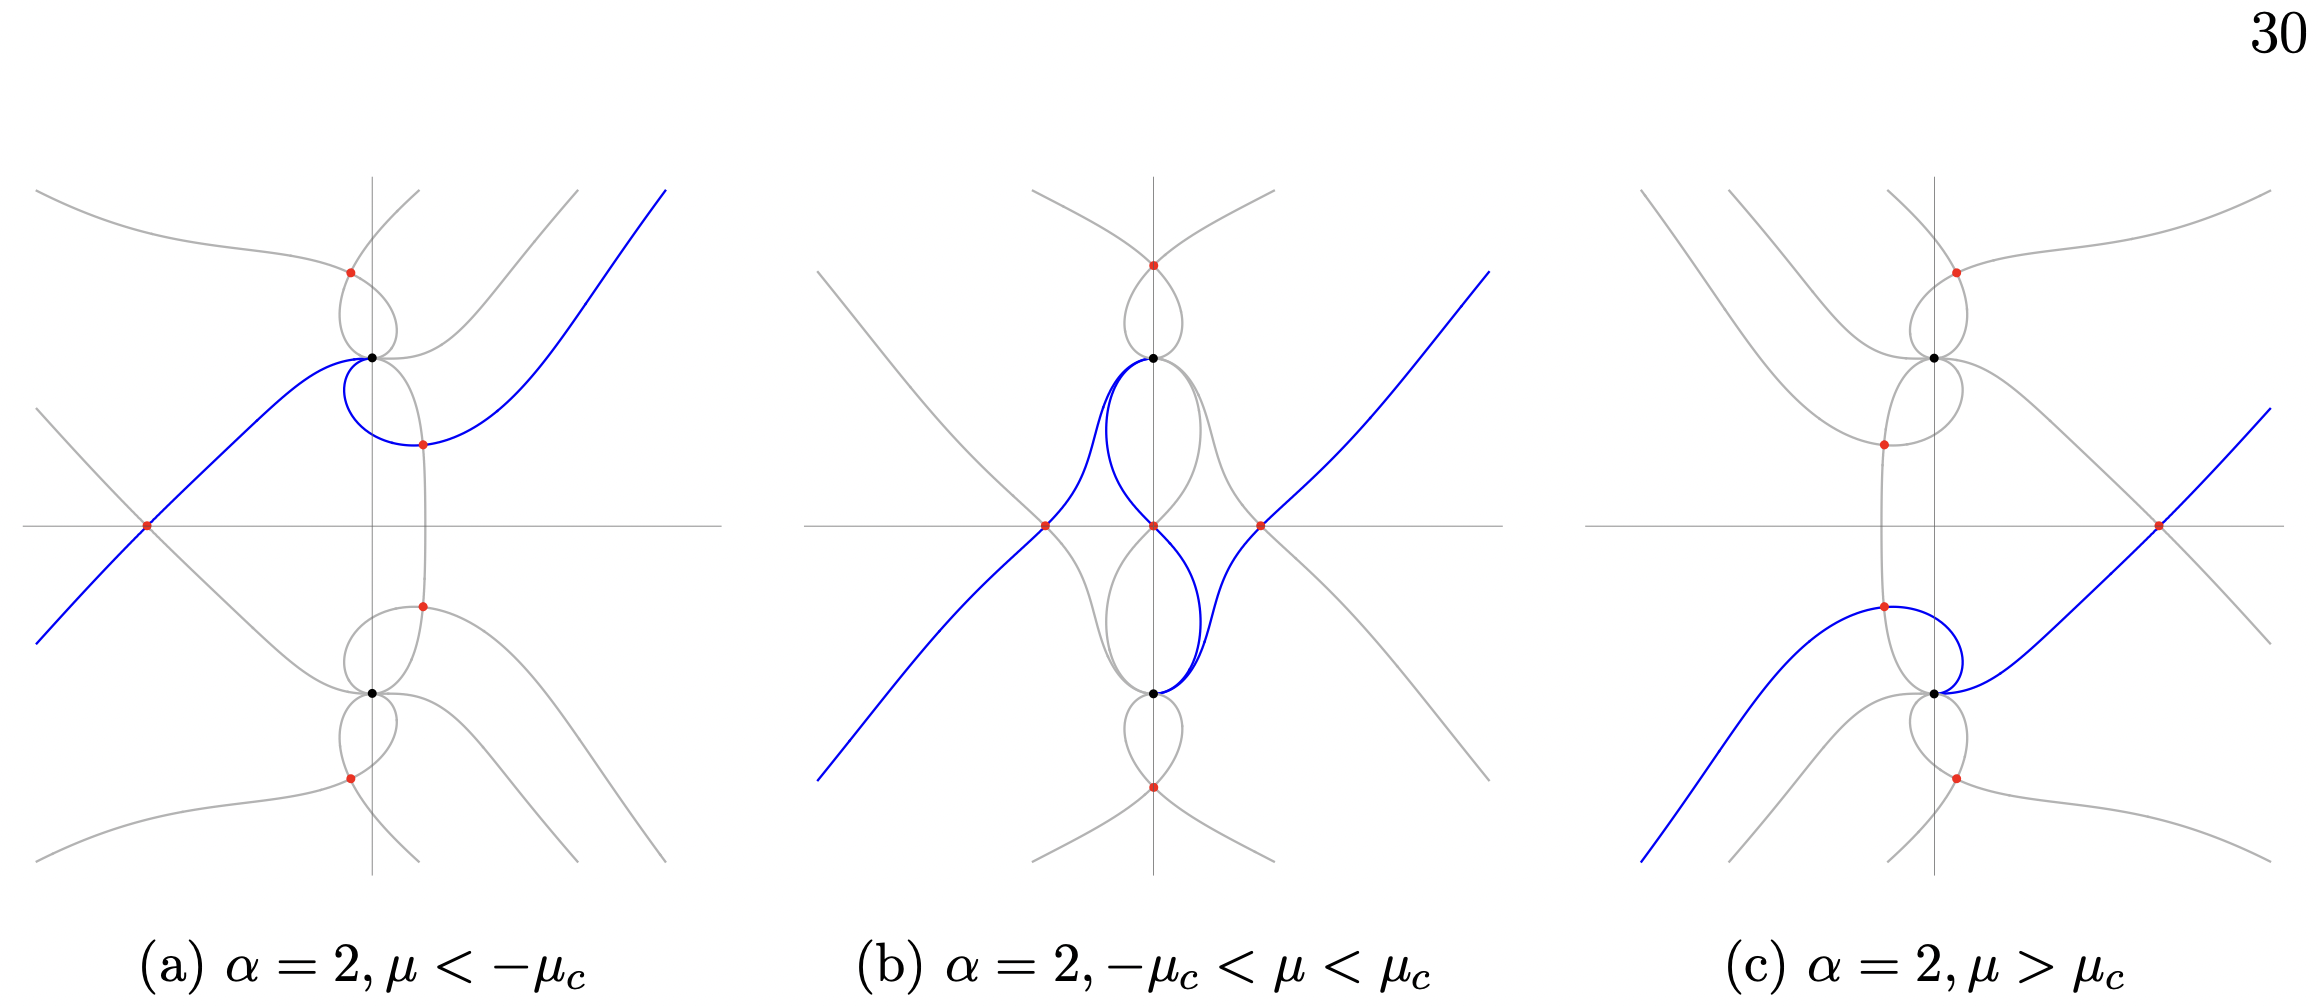
\includegraphics[width=4.5in]{Figures/thimbles.png}

Feldbrugge+2019
  }



  \frame{
\vspace{-0.5in}
    \frametitle{New Observables}
    \begin{itemize}
    \item for coherent sources: FRBs, pulsars
    \item weak lensing: effervescent image allows time delay measurement (Jow+21)
    \item microlensing: instant time delay, planets (Jow+20)
    \item macrolensing: potentially nano-second delay -- universe
      expands!  Dark energy, etc (Wucknitz+21)
    \item dimensionless strain cm/Gigalightyears $h\sim \Delta t/t \sim 10^{-26}$:
      competitive with LIGO, etc
    \end{itemize}
  }



  \frame{
%\vspace{-0.25in}
    \frametitle{Macro lensing}
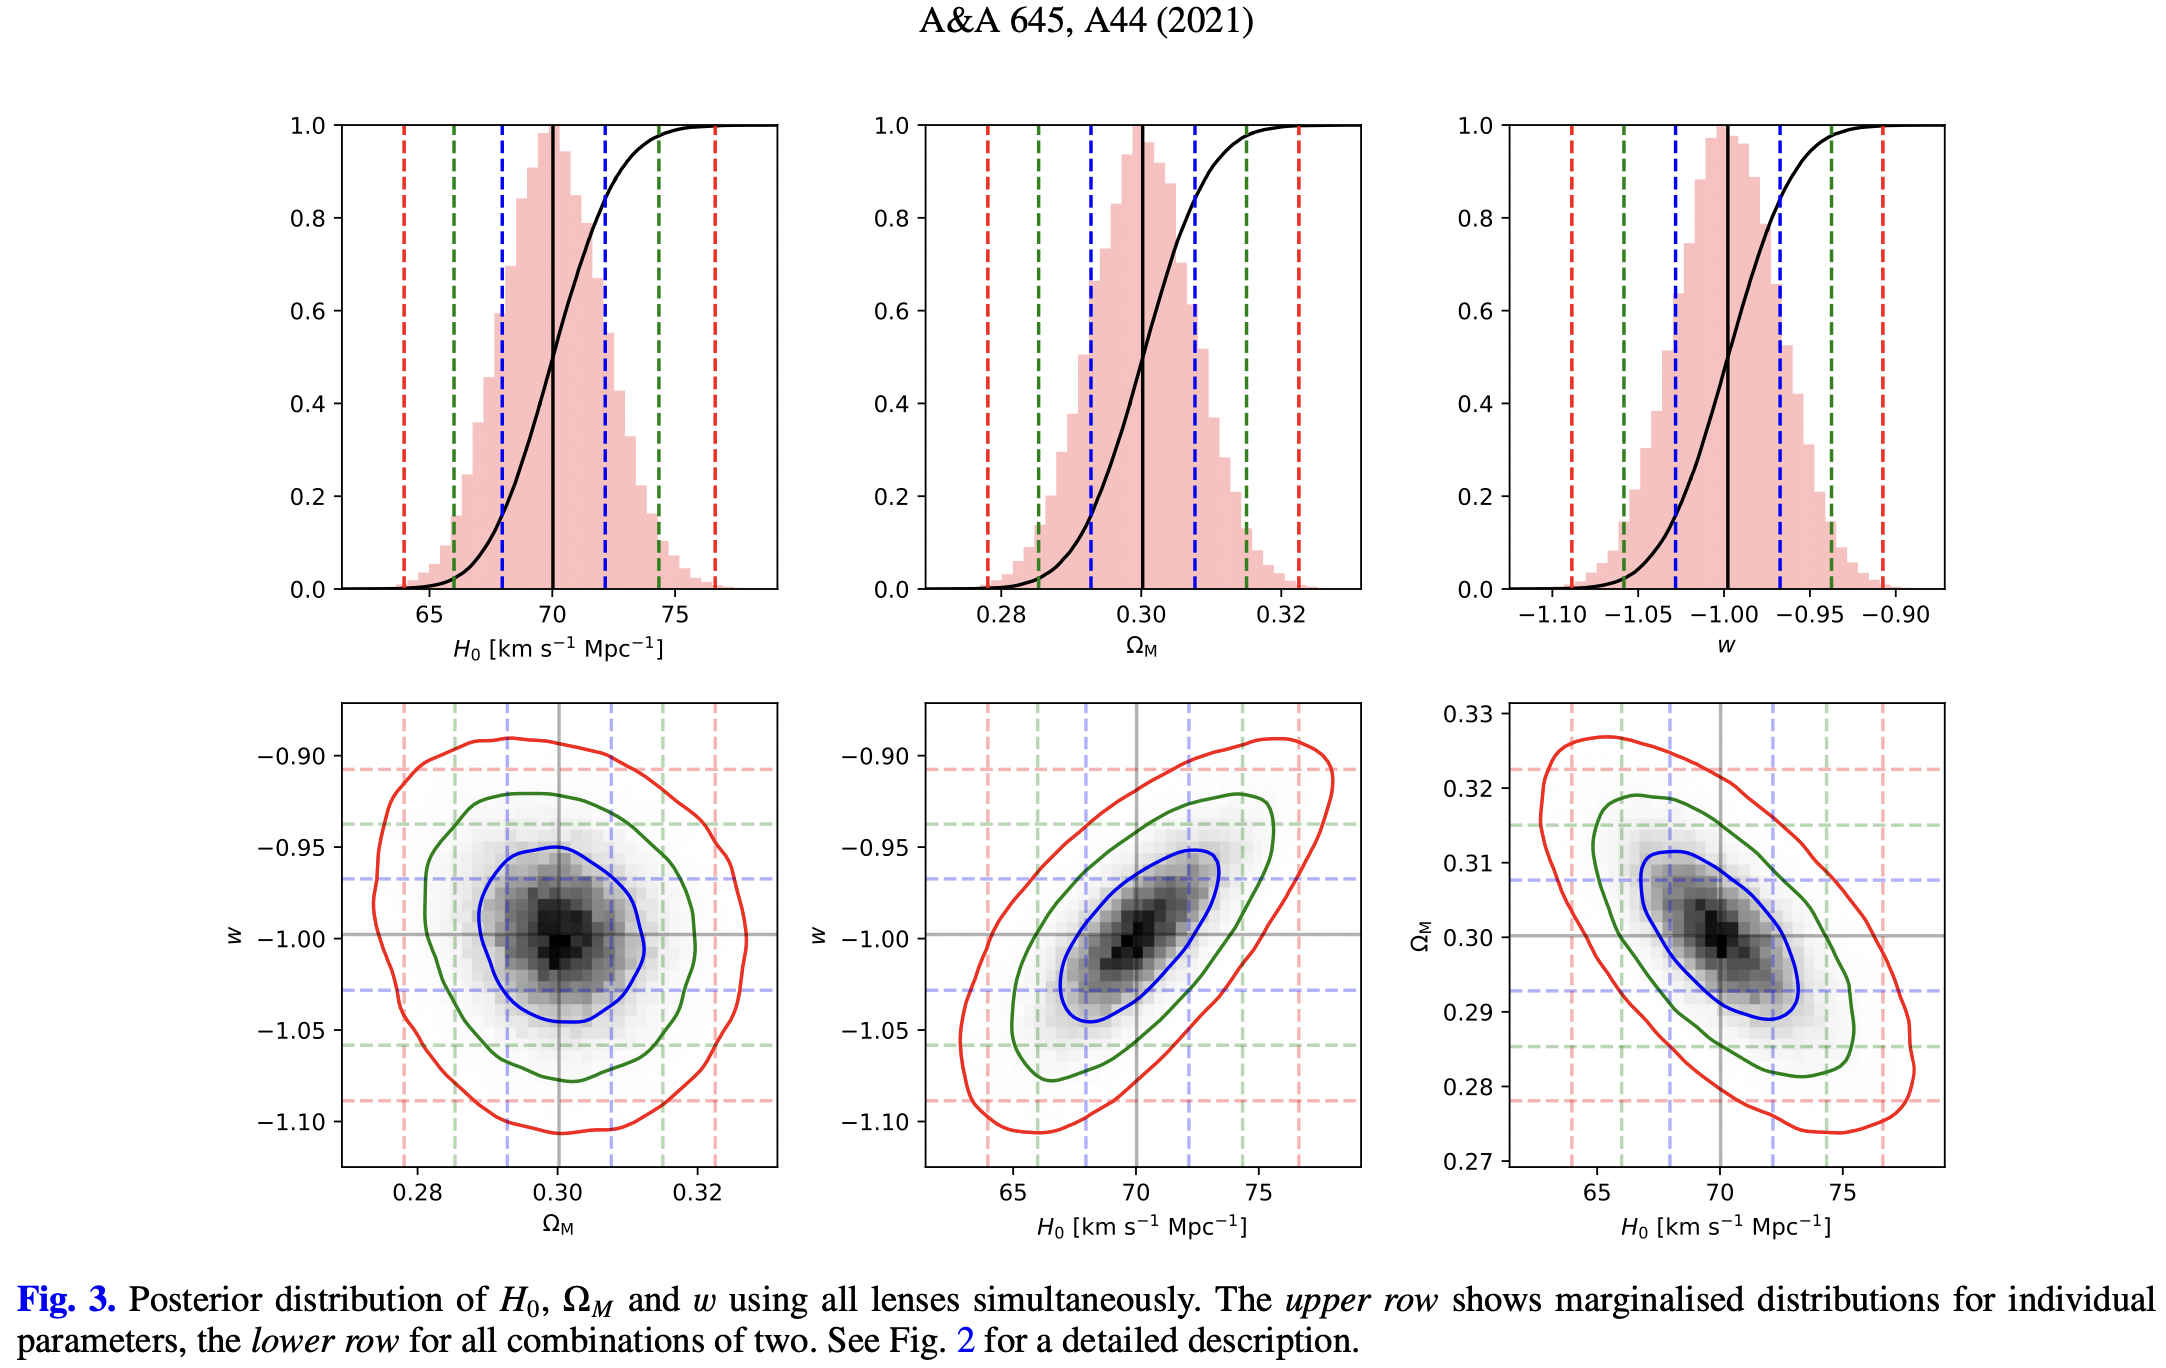
\includegraphics[width=4.5in]{Figures/wucknitz.png}

Wucknitz, Spitler, ULP 2021, A\&A, 645, A44
  }





  \frame{
    \frametitle{Diffractive/Effervescent Gravitational Wave Lensing}
\includegraphics[width=4.5in]{Figures/PTAGWLensing.pdf}

Jow+ in prep
  }


  \frame{
\vspace{-0.5in}
    \frametitle{Discussion}
    \begin{itemize}
    \item Eikonal effects applicable to compact radio sources,
      e.g. FRBs, pulsars
    \item full wave
effect dominates for long wavelengths as Fresnel scale is bigger then Einstein radius
    \item microlensing down to planet size
    \item gravitational waves:  LIGO, LISA, PTA
    \end{itemize}
  }

  \frame{
\vspace{-0.5in}
    \frametitle{Quantum Mechanics}
    \begin{itemize}
    \item Feynmann path integral saddle points are similarly complex
    \item interprets tunneling as complex position path
    \end{itemize}
  }

  \frame{
%\vspace{-0.5in}
    \frametitle{Rosen-Morse Potential}
\begin{itemize}
\item $V(x)={\rm sech}^2(x)$
  \item  exactly solvable: 
$\sinh[x(t)]=\sqrt{\frac{1-E}{E}} \cosh[\sqrt{E}(t+t_0)]$
    \item for $\lim_{E\rightarrow 1+\epsilon^2} = \sinh^{-1} [\epsilon \sinh(t)]$
    \end{itemize}
 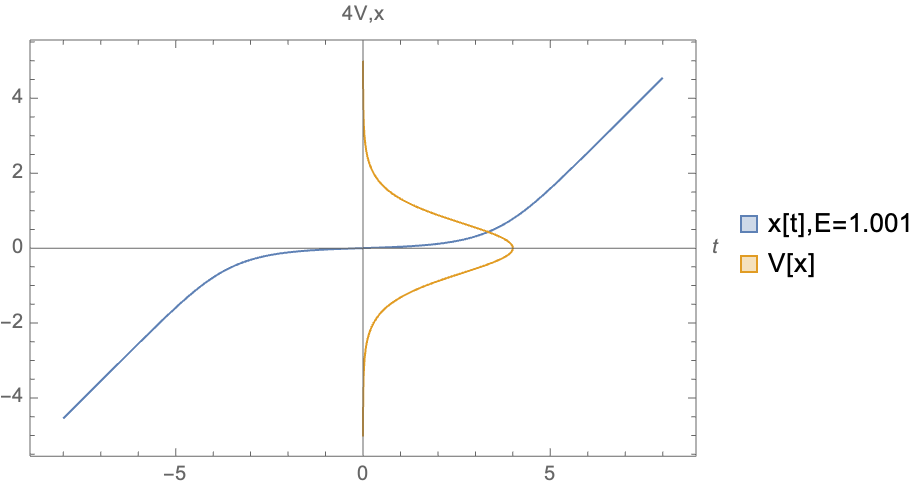
\includegraphics[width=3.5in]{Figures/sechreal.png}
  }


  \frame{
\vspace{-0.5in}
    \frametitle{Rosen-Morse Potential}
\begin{itemize}
\item $V(x)={\rm sech}^2(x)$
  \item  exactly solvable: 
$x(t)=-i \sin^{-1}\left[\sqrt{\frac{1-E}{E}}\sinh(\sqrt{E}t)\right]$
    \item for $\lim_{E\rightarrow 0} = -i\sin^{-1}(t)$
    \end{itemize}
 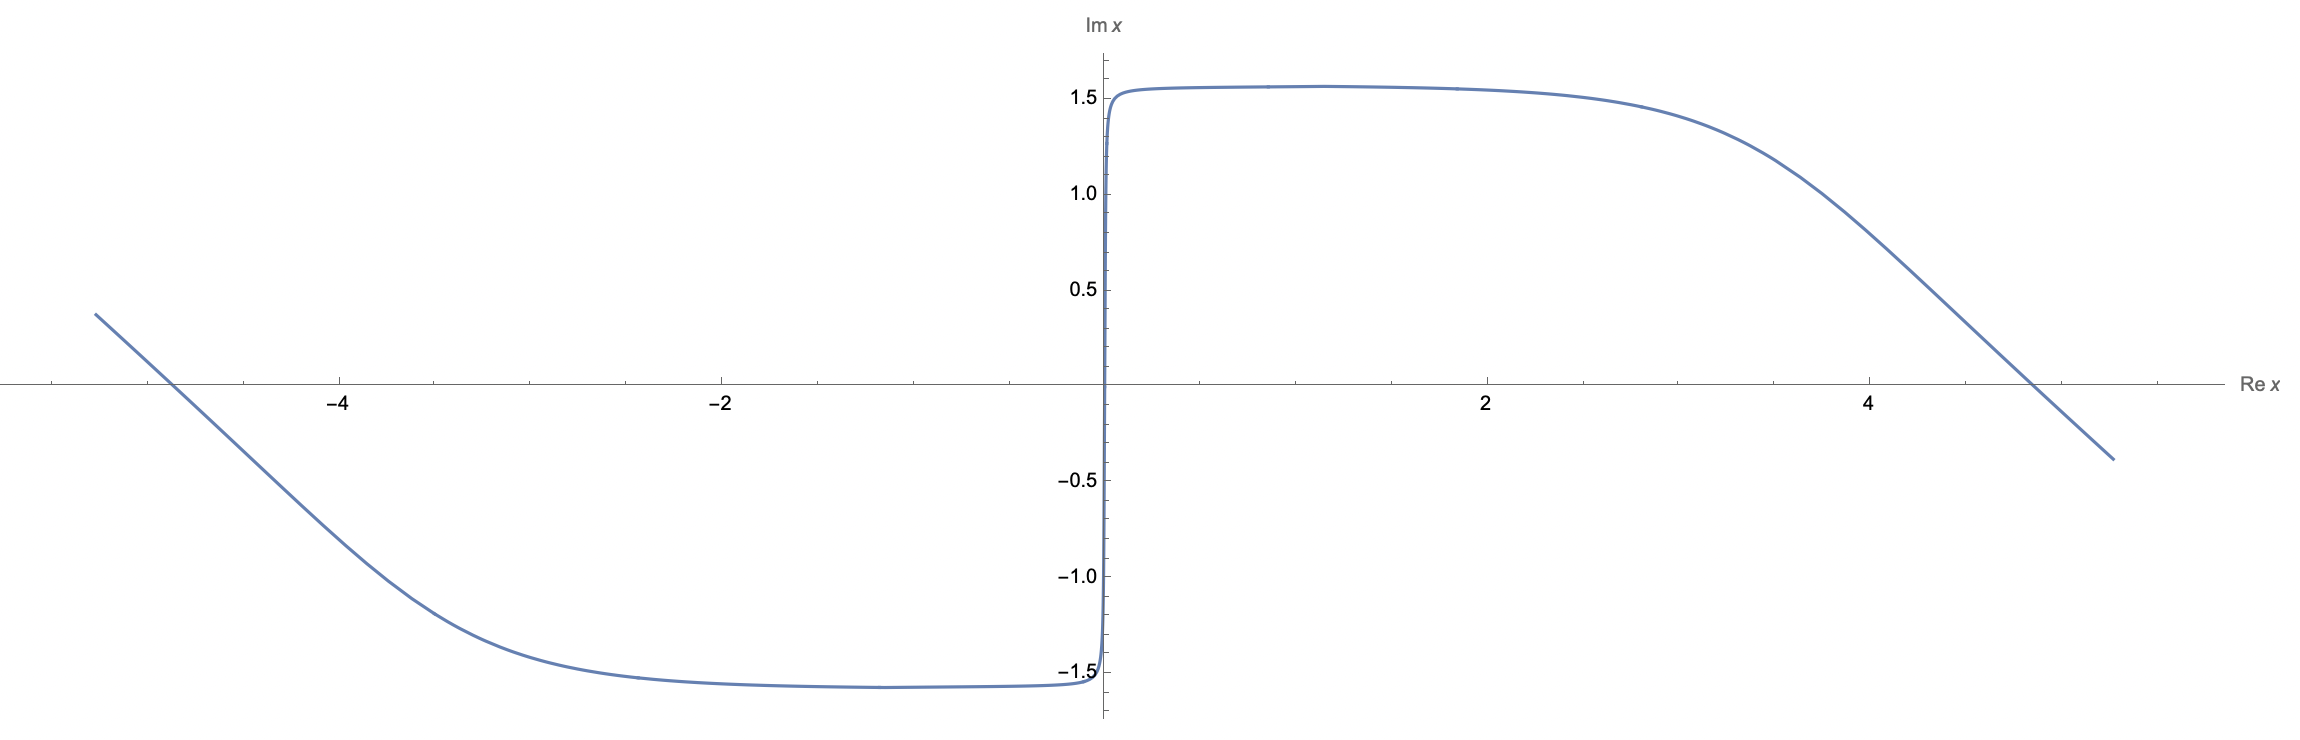
\includegraphics[width=4.5in]{Figures/sechtunnel.png}
  }



  \frame{
\vspace{-0.15in}
    \frametitle{Reinterpretation of Quantum Mechanics: 2309.12420 w/Feldbrugge, Jow}
\begin{figure}
        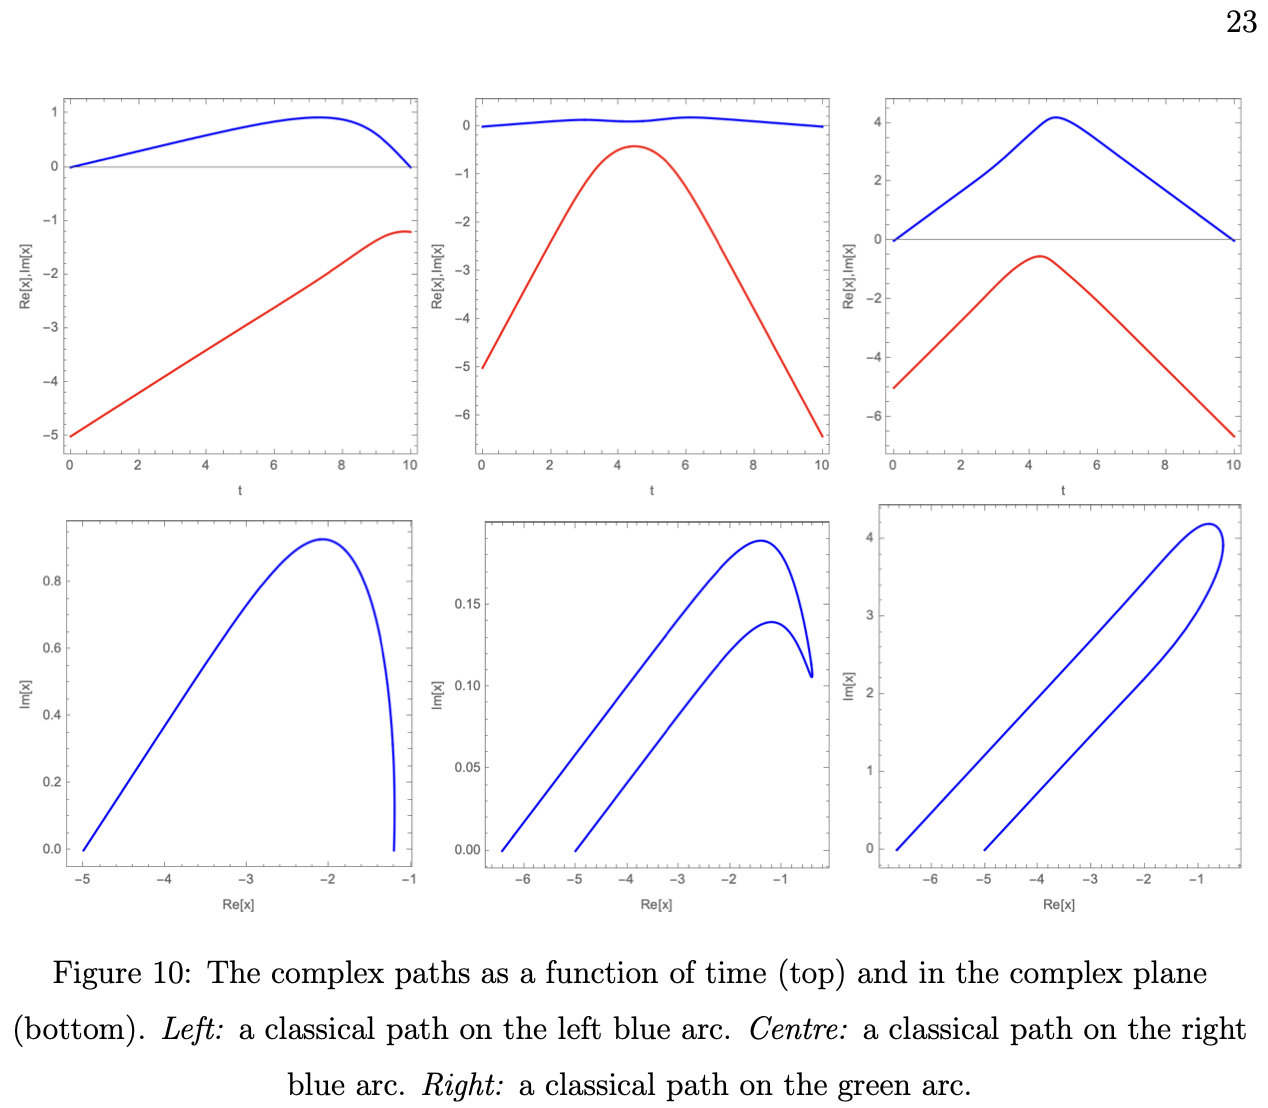
\includegraphics[width =0.8\textwidth]{Figures/saddle.png}
\end{figure}


  }




  \frame{
%\vspace{-0.5in}
    \frametitle{Conclusions}
    \begin{itemize}
     \item wave optics changes nature of astrophysical observables: Coherent FRB/pulsar/GW      radiation one of the potentially most
      precise measurements in physics
      \item already makes microarcsecond images of pulsars
      \item ISM plasma screens modelled quantitatively as localized
        1-D features, no longer stochastic turbulent volume.
    \item Picard-Lefschetz theory provides alternative interpretation
      of optics, quantum mechanics: imaginary positions and trajectories
      \item next generation FRB telescopes for cosmic mass inventory,
        possibly dark energy/acceleration
      \item PTA weak diffractive lensing may give new tool for Hubble
        Constant tension
    \end{itemize}
  }

\end{document}
